\subsection{UC7 - Posizionamento scaffalatura}
\begin{figure}[H]
  \centering
  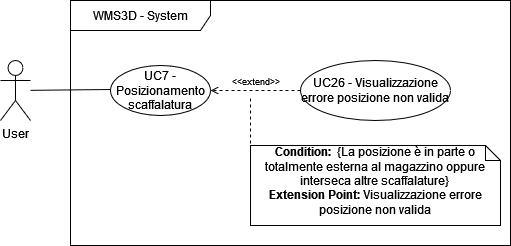
\includegraphics[width=0.8\textwidth]{UC_diagrams_1-10/UC7.drawio.png}
   \caption{Diagramma UML UC7 - Posizionamento scaffalatura}
\end{figure}
\begin{itemize}
    \item \textbf{Attori:} User.
    \item \textbf{Pre-condizione:}  L'utente ha creato una scaffalatura [UC6] e sta visualizzando il magazzino in 3D [UC3].
    \item \textbf{Post-condizione:} La scaffalatura creata è posizionata all'interno del render 3D.
    \item \textbf{Scenario Principale:} L'utente dopo aver creato una scaffalatura sceglie dove e come posizionarla all'interno del magazzino.
    \item \textbf{Generalizzazioni:} -
    \item \textbf{Estensioni:} È presente una estensione nel caso in cui la posizione non sia valida:
    \begin{itemize}
        \item UC26 - Visualizzazione errore posizione non valida.
    \end{itemize}
\end{itemize}